% !TEX root = ../thesis.tex
\chapter{Results and Discussion}
\label{chap:results}

We will first look at the web application results based on the user's feedback, and then we will look into the insights and potential feedback the NLP process could provide the user. We then also look to review the overall process. 

We will compare the web application's results against the comparative judgment, Elo ranking, and the score we created for the tweets on Twitter. With the insights of the NLP for feedback to the user, we will look at what insights got made. Additionally, we will look at if any of the knowledge extracted generated provides any meaningful feedback to the user.



\section{Tweet Ranking Results} 
\label{sec:reaults_ranking}

	\begin{figure}[h]
		\centering
		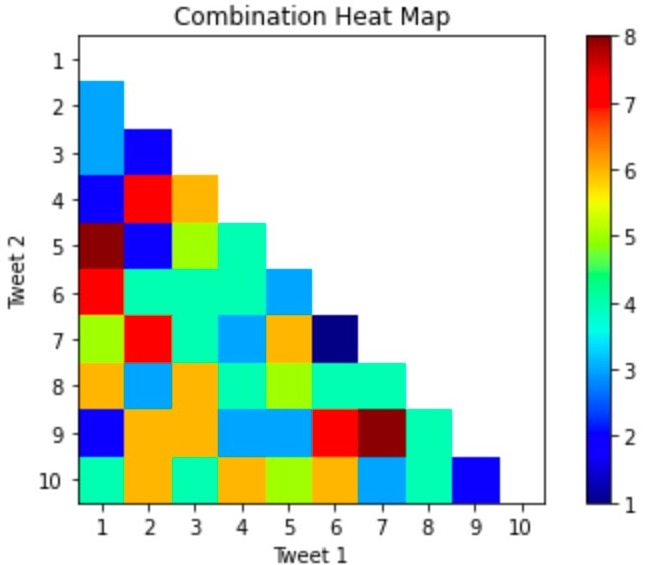
\includegraphics[width=7cm]{combination_heat_map.png}
		\caption{The web applicaitons generated results compared agaist each other.}
		\label{fig:combinations}
		
	\end{figure}
	
	Forty different users take part in the comparison judgement within the web app. Through looking at fig: \ref{fig:combinations} we can see that all combinations got displayed to the users taking part in the comparisons. We can see that tweet one and tweet five appeared the most, while the combination appearing the lowest was tweet six and seven, with one comparison getting presented to the users.
	
	\begin{figure}[t]
		\centering
		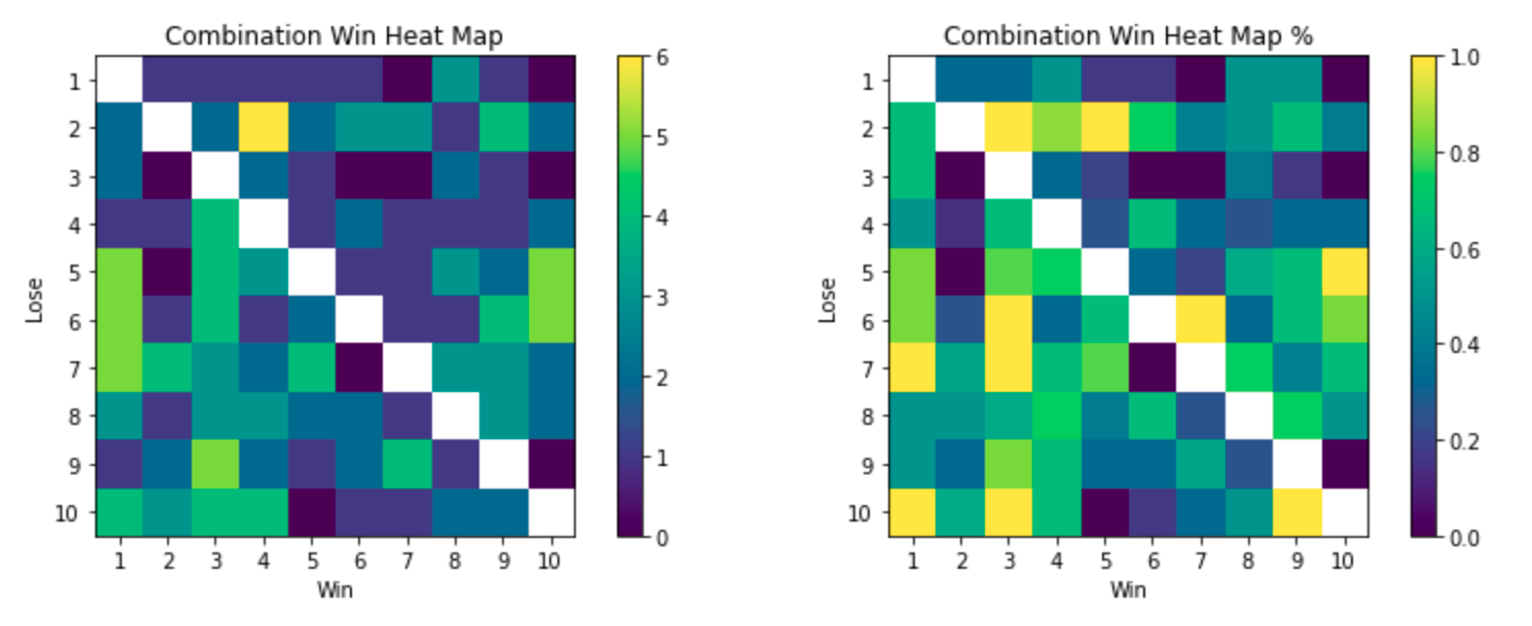
\includegraphics[width=\textwidth]{Combination_win_with_perc_heat_map.png}
		\caption{A heat map of the amount of times a tweet win or lost. Left - by total values. Right - By win percentages.}
		\label{fig:Combination_win_with_perc_heat_map}
		
	\end{figure}
	
	\begin{figure}[b]
		\centering
		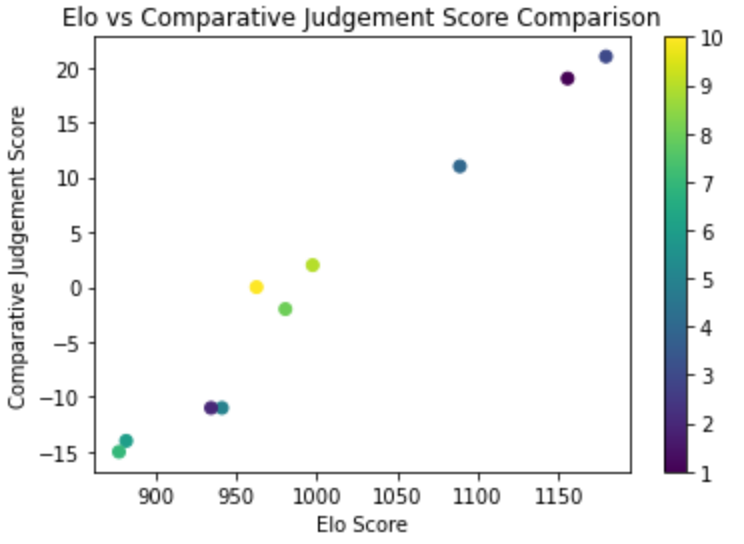
\includegraphics[width=7cm]{elo_vs_cj_comparison.png}
		\caption{A scatter graph plotting each tweet againast their Elo and comparative judgement score.}
		\label{fig:elo_vs_cj_comparison}
		
	\end{figure}
	
	When we look at winners and losers of the comparisons (see fig: \ref{fig:Combination_win_with_perc_heat_map}), we can see that the tweet that won the most between a specific combination was tweet four and two, with tweet four winning six times and tweet two winning only once. Additionally, when we look at the combination that appeared the most, one and five, one came out on top five times, compared to five winning between the two once.
	
	When we look at the winner heat map (see fig: \ref{fig:Combination_win_with_perc_heat_map}), we can see that two, five, six, seven and ten had moments where they didn't win a head-to-head with another tweet. Two, six, seven and ten didn't win against at least two different tweets, while the others were only against one tweet they failed to win. We can see that certain tweets never won against another tweet. For example, Tweet 10 never beat Tweet 9, which is also reflected in the ranking of the tweets, as Tweet 9 is ranked higher than Tweet 10 in both the Elo and CJ ranking table. The same can get said about Tweet 6 and 3, with Tweet 6 never beating Tweet 3, and Tweet 6 came 9th, and Tweet 3 came 1st in the rankings.
	
	%\begin{figure}[h]
	%	\centering
	%	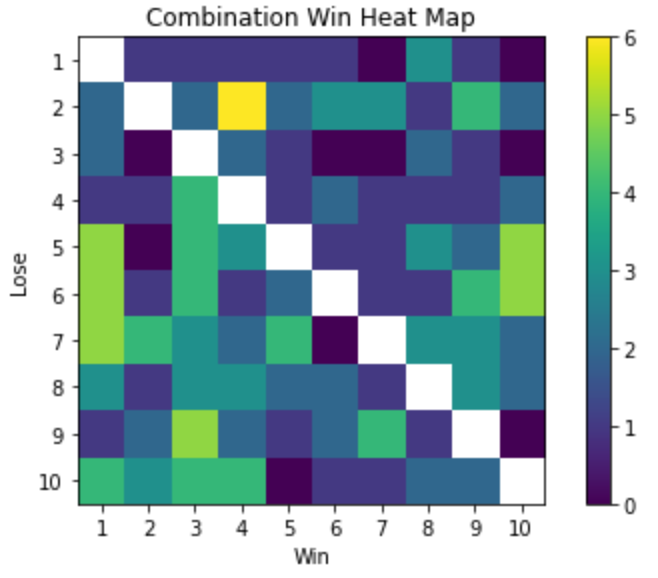
\includegraphics[width=7cm]{combination_win_heat_map.png}
	%	\caption{A heat map of the amount of times a tweet win or lost.}
	%	\label{fig:combination_wins}
		
	%\end{figure}
	
\begin{figure}[t]
	\centering
	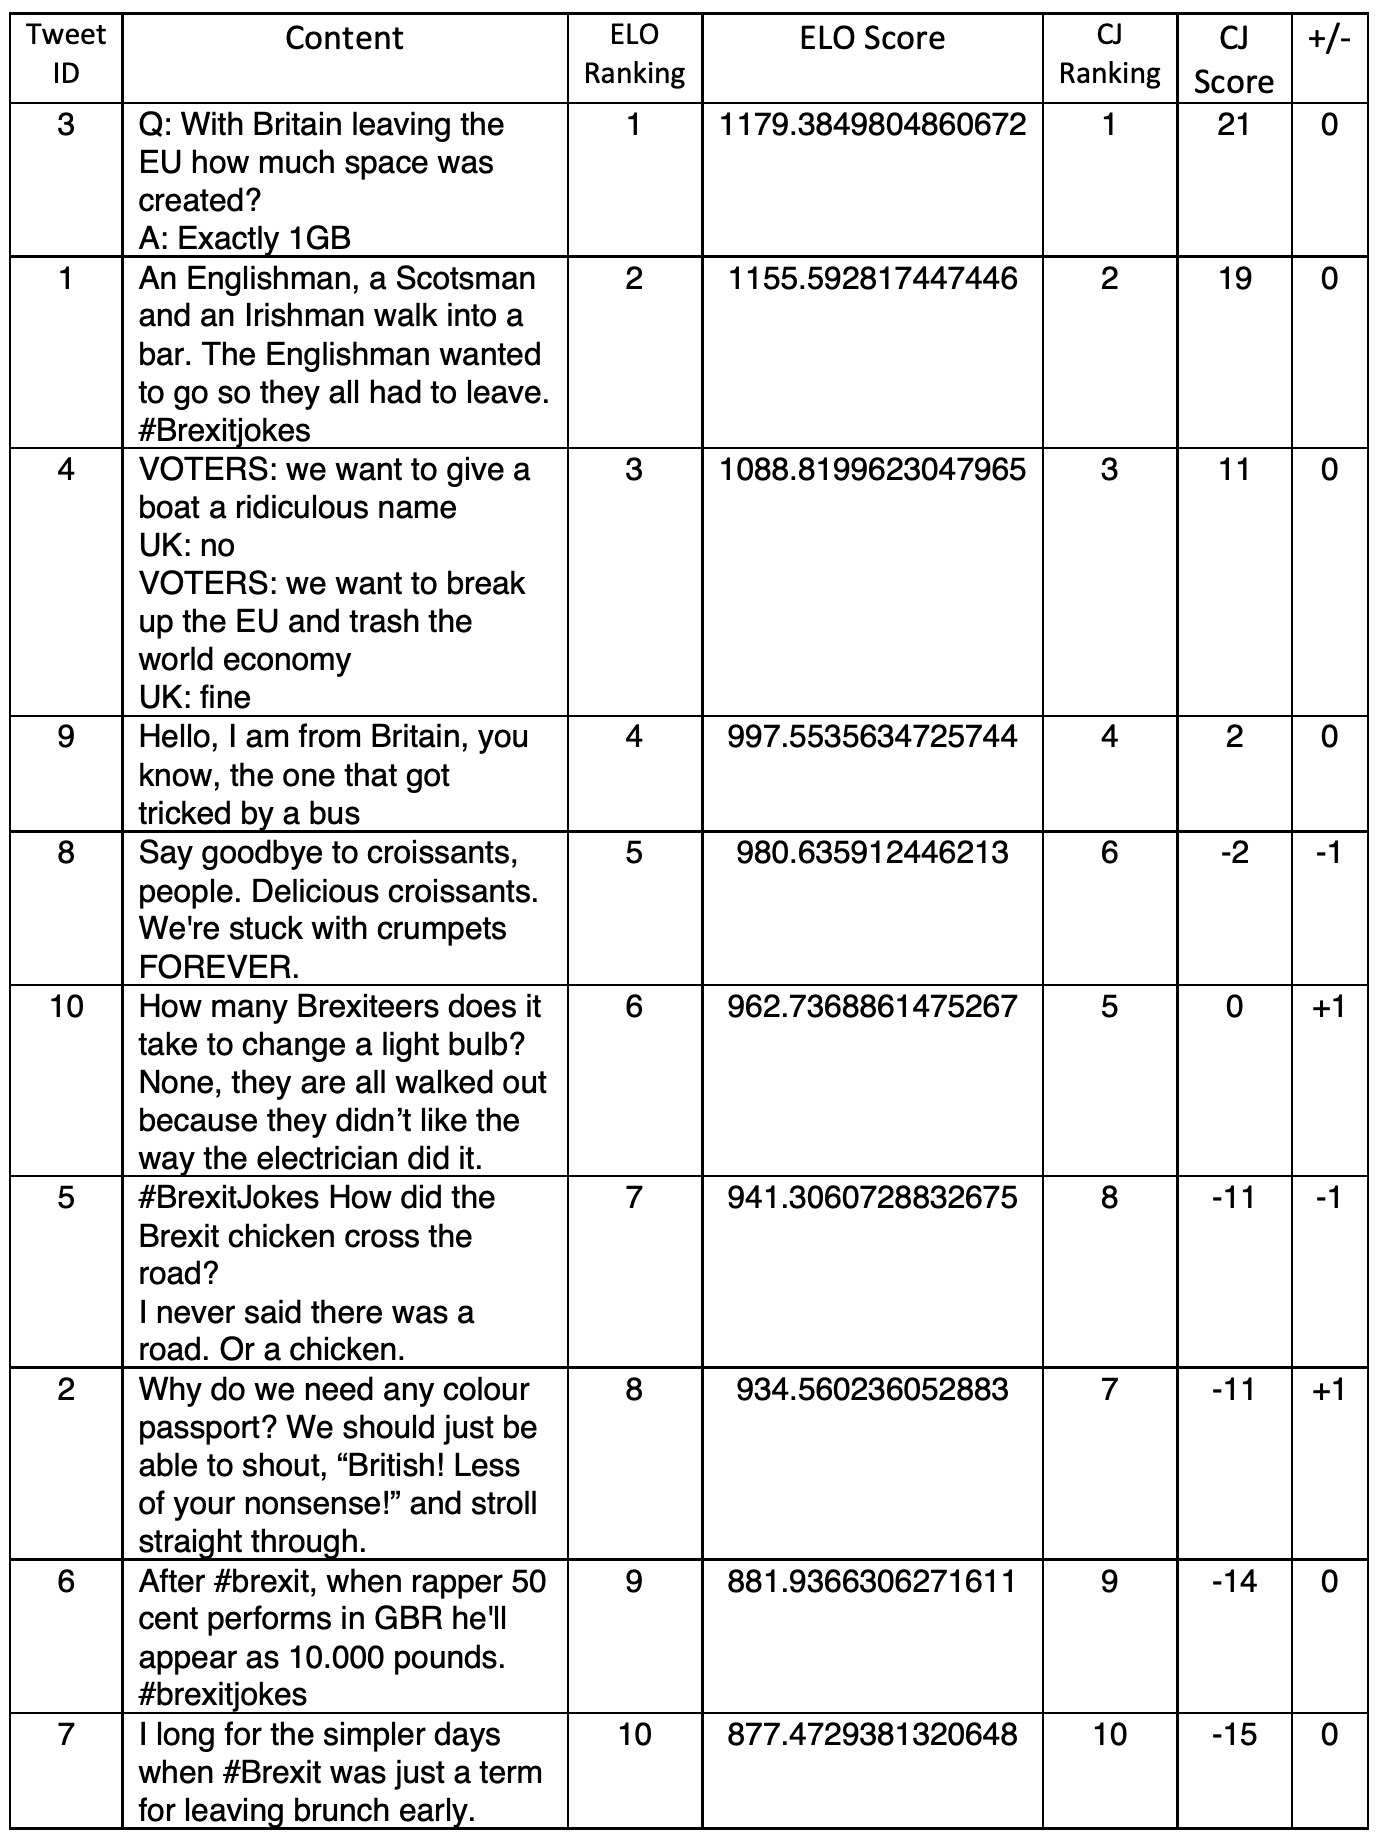
\includegraphics[width=10cm]{web_app_results.png}
	\caption{The web applicaitons generated results compared agaist each other.}
	\label{fig:web_app_results}
	
\end{figure}
	

	When we look at the two scores plotted against each other, Elo and CJ (see fig: \ref{fig:elo_vs_cj_comparison}), it shows that these values are linearly correlated. Additionally, the results returned as 0.98391595 when a Pearsons correlation test got conducted on these scores. Therefore, the two values are heavily linked, so when a tweet has a good Elo score, it also has a good CJ score. This correlation between the results shows that the Elo score is an excellent alternative to the CJ scoring system. Through using the Elo system, also provides the process with a lot more robustness. It allows the ranking to get done to a high degree of accuracy. Additionally, without every combination getting presented against each other. As a result, this would be a sound scoring system to implement at a national scaled-up scale.

	While looking at fig \ref{fig:web_app_results}, we can see that the Elo and comparative judgement ranking generated very similar results. However, as we can see, the tweets coming in 6th, 7th, and 8th slightly vary in the results. These CJ results bring about some questions about whether further work is required to rank them more accurately. However, we need to ensure that the process does not end up having someone do multiple rounds and then expand the time required to complete the CJ, taking away any actual benefits. But it does bring to light how effective the Elo ranking system is and can handle these situations. It takes a score calculation based on the likelihood that the tweet will win, rather than a more dogmatic approach of the total wins minus the total losses.
	
	\begin{figure}[t]
		\centering
		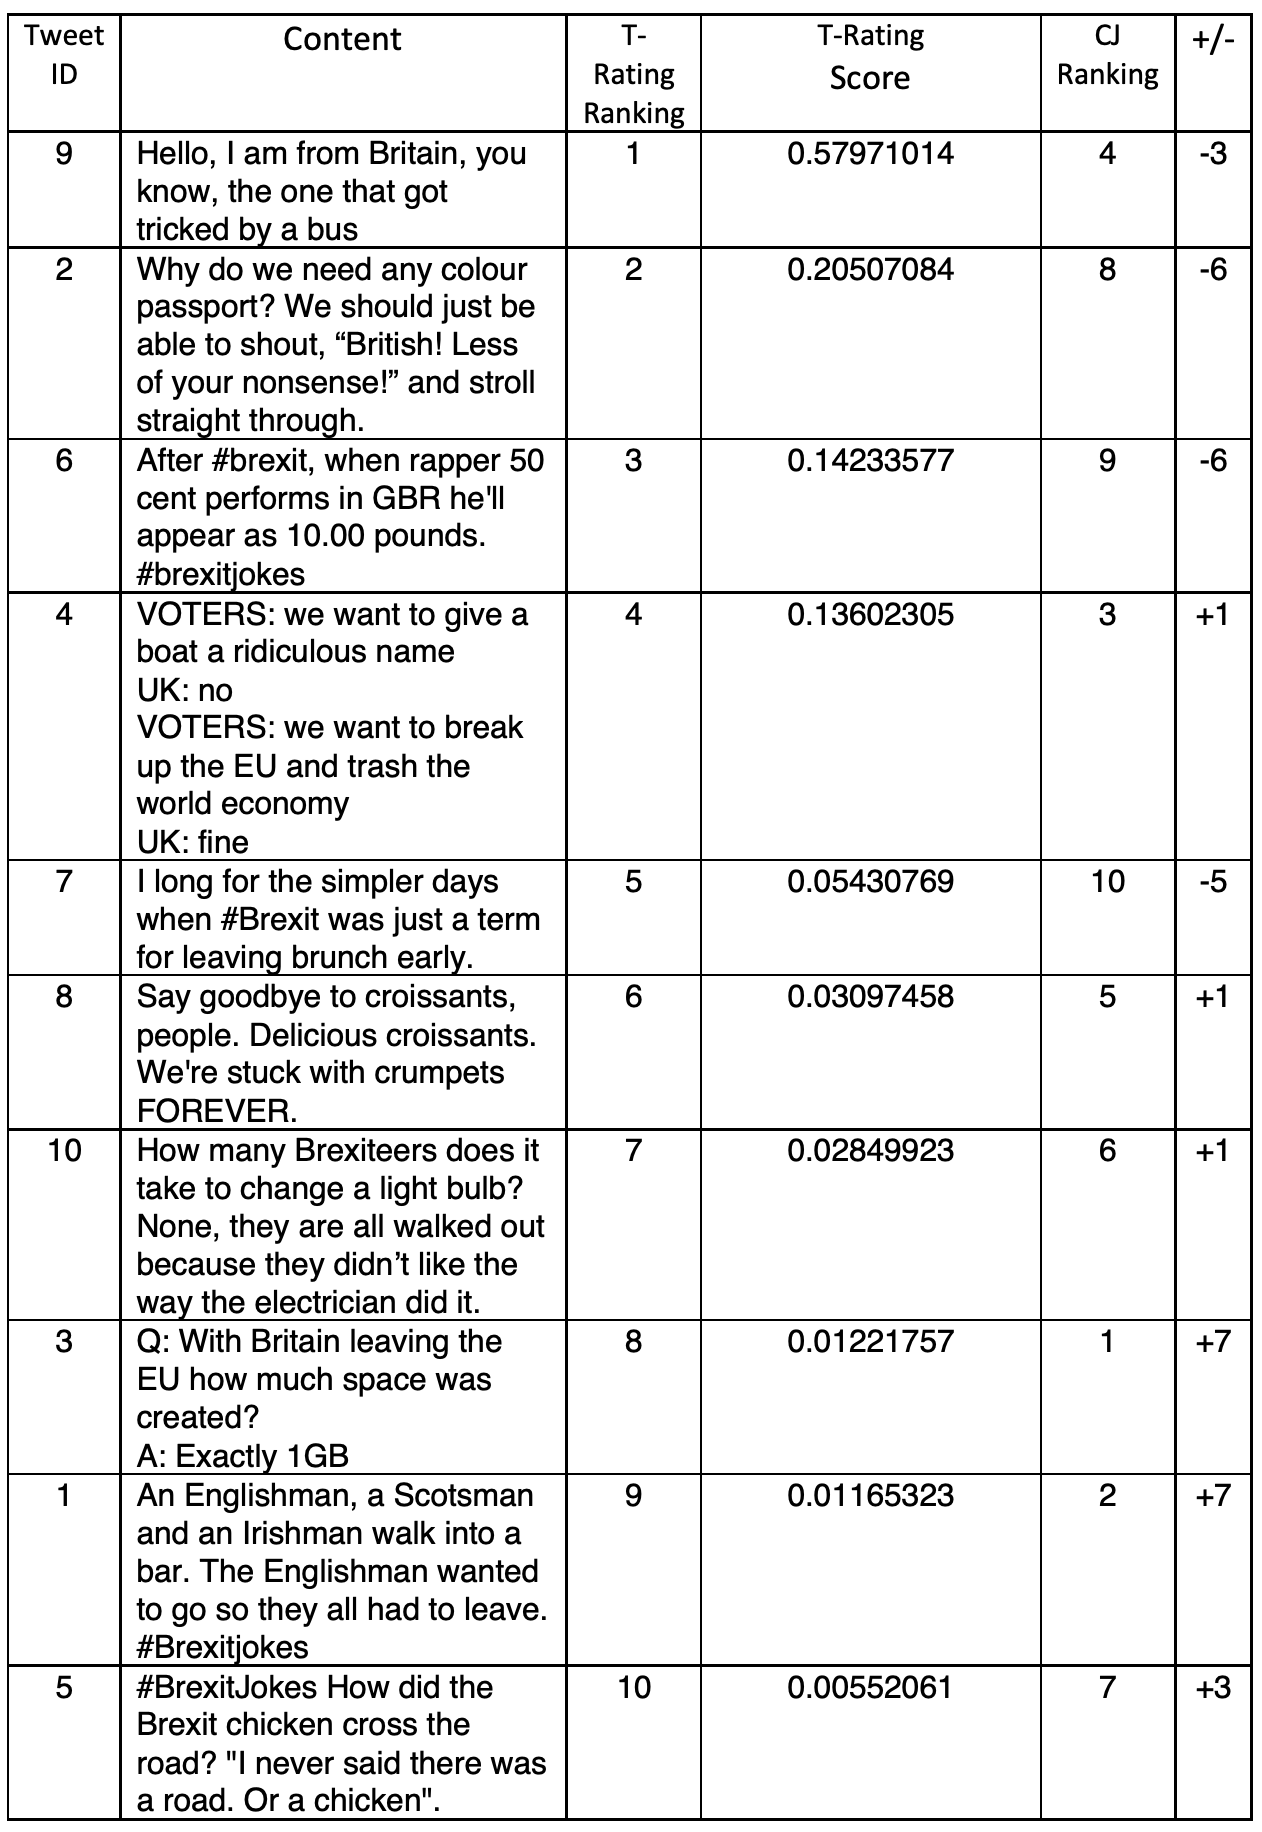
\includegraphics[width=10cm]{twitter_results_comparison.png}
		\caption{The Twitter tweet score ranking comparison against Elo ranking.}
		\label{fig:twitter_results_comparison}
		
	\end{figure}

	\begin{figure}[t]
		\centering
		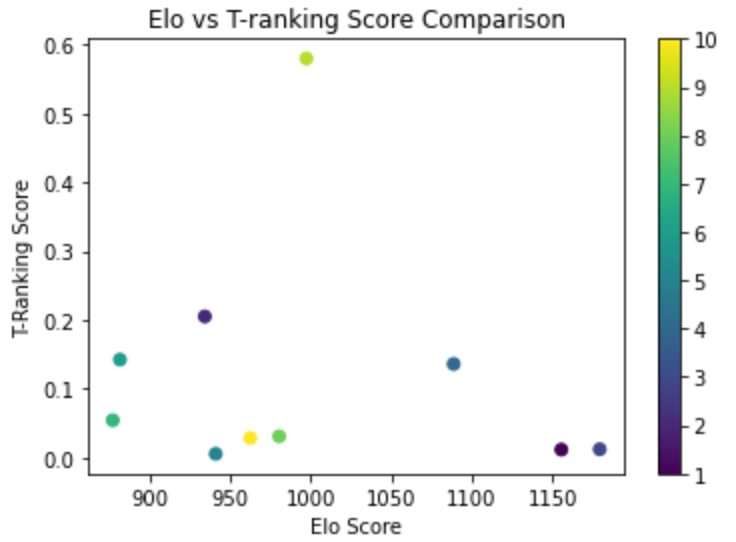
\includegraphics[width=10cm]{elo_vs_tr.png}
		\caption{The Twitter tweet score ranking plotted against Elo ranking.}
		\label{fig:elo_vs_tranking}
		
	\end{figure}

	While we look at the T-rating ranking compared to the Elo ranking (see fig: \ref{fig:twitter_results_comparison}), we can see that the results ranking is very different. The tweet that came first in the T-rating came fourth in the Elo ranking. At the same time, the tweet that came first in the Elo ranking came eighth in the T-rating.  Tweets that done worse in the Elo ranking compared to T-rating had an average difference in the ranked placing of 5 places, while the tweets that had a better Elo ranking compared to the T-ranking ranked an average of 4 places lower. Therefore, 4 of the top 5 tweets in the T-rating were actually in the bottom five of the Elo ranking. Only tweet ID 4 done one place better with the Elo ranking than it did in the T-ranking. However, two of the top three tweets in the T-rating were in the bottom three of the Elo ranking and vice versa. The T-rating score has a correlation score of -0.14360792 against Elo and -0.09776676 against CJ. They were showing us that there is a negative correlation between the scores. It does make it seem like how popular something is on Twitter doesn't mean it is necessarily a funnier tweet when carried out in a controlled environment.
	
	However, even though these ended up with very different results (see fig: \ref{fig:elo_vs_tranking}), due to the multiple variables at play regarding Twitter, in terms of likes, retweets, followers, how many followers retweeters have, a tweet might have, the random chance of someone seeing it. The T-rating system is a very ambiguous metric to use as an accurate ranking system. Additionally, with Twitter being a global app, the results on certain tweets could be affected by people's views from outside the UK, drastically changing opinions. Another factor that is making this a difficult comparison to make is the sample size. The tweets on Twitter had many more people interacting with them than how many people took part in our study. Therefore, how the tweet did in the real world is not a valid comparison against the Elo rankings results. There is also room to suggest that this proves that the Elo system is better suited for this action, as it can handle random elements of its pairings. 
	
	However, this comparison has brought to light a valid point: do we want the results to be decided upon by a local group of specialised people? Or do we want the results to get agreed upon as a global element? For example, teachers within a school in the UK would possibly be looking for different work factors compared to a teacher in Finland. Therefore, creating contrast in views. Additionally, GCSE awards bodies might also have different focuses within their assessments, even when it comes to subjects like English. So this could have a huge impact on views getting generated around the ranking of students work which would need further investigating.

	Within the forty participants, twenty-two of them left a justification for why they select one tweet over the other. However, the participants' responses were varied in the amount of provided feedback. Some proved a justification for all five combinations. On the other hand, some only left them for a few and not all. The users gave a total of sixty-three explanations to their decisions on which tweet they had chosen.
	
	One user stated, "I just think it is a clever way to put our departure from EU, plus it did make me giggle." The comment was in regards to tweet three beating tweet eight. Tweet three did provide several justifications, a lot of them to do around its tech theme on Brexit. Some of the rationales are "Comp sci wordplay", "everyone loves a tech joke", "Because it's the nerdier option", the "First tweet just lol", and "Actually laughed out loud".
	
	Another tweet, tweet ten beating tweet 8, had the justification for winning as 'because of the wordplay'. So we can see that several tweets had some form of explanation around the lines of good wordplay. Therefore, creating user feedback has not made an excellent source of information to help build feedback. However, it has given some context to why they had made their decisions.


\section{NLP Feedback and Insights}
\label{sec:reaults_NLP}
	
	The Jupyter notebook was able to conduct the NLP tasks that we required successfully. We presented the user the POS tagging insights of how many POS tags were present in each tweet. We were also able to visualise the POS tagging to reflect the user how the tweet got broken down structure-wise (see fig: \ref{fig:POS_example}).
	
	\begin{figure}[h]
		\centering
		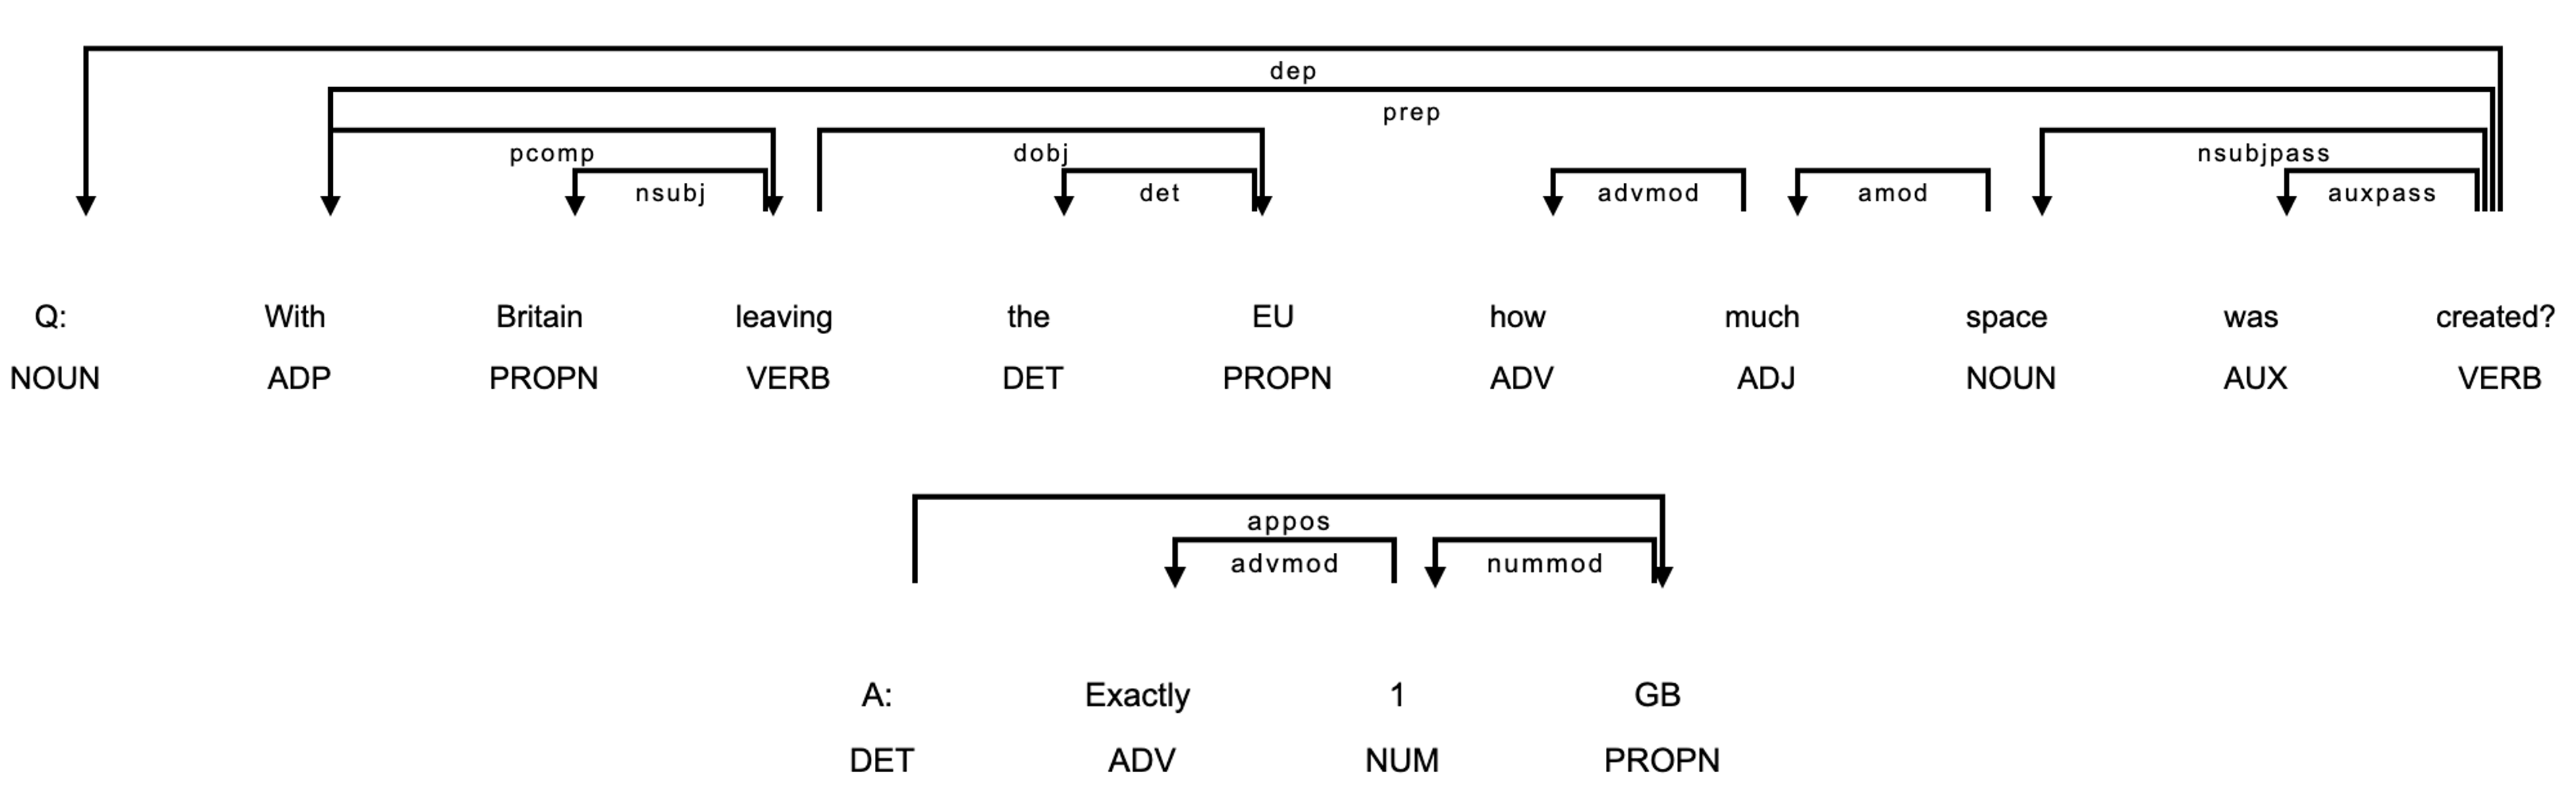
\includegraphics[width=\textwidth]{POS_vis.png}
		\caption{An example of a POS tagging visulaisation. To see all the outputs, please look at appendix: \ref{app:POS_vis}}
		\label{fig:POS_example}
		
	\end{figure}

	We were also able to present to the user the NER that the pre-trained model supplied by spaCy was able to identify. These were presented to the user in text format as well within a visualisation, identifying the NERs within the sentence (see fig: \ref{fig:NER_example}).
	
	\begin{figure}[h]
		\centering
		
\includegraphics[width=\textwidth]{NER_vis.png}
		\caption{An example of a NER tagging visulaisation. To see all the outputs, please look at appendix: \ref{app:NER_vis}}
		\label{fig:NER_example}
		
	\end{figure}

	The notebook was also able to present back to the user the top ten tweets on how similar they were by the whole tweet (see fig: \ref{fig:top_10_sim_doc}) and by NERs (see fig: \ref{fig:top_10_sim_NER}). When looking at the results for the similarity scoring between the NERs, we can see that the most similar tweets are tweet three and tweet 4. These tweets have a similarity score of 0.857896 based on the NER values Britain, EU (Tweet 1) and UK, EU (Tweet 4). The tweets with the least similarity are Tweet 2, British, and Tweet 6, 50, cent, 10.00, pounds, with a similarity score of -0.025753.
	 
	
	\begin{figure}[h]
		\centering
		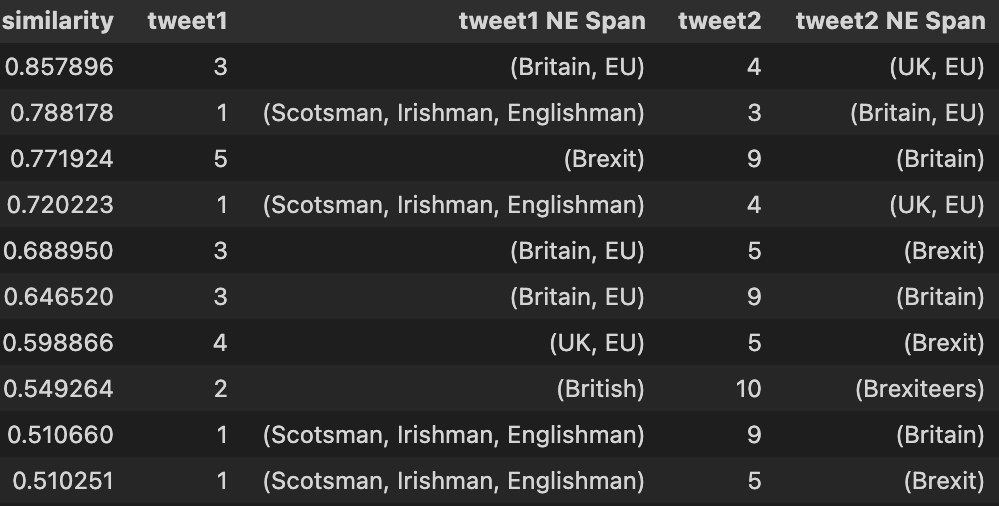
\includegraphics[width=10cm]{top_10_sim_NER.png}
		\caption{A table displaying the top ten similar tweets based on the tweet's NERs.}
		\label{fig:top_10_sim_NER}
		
	\end{figure}

	The results show us, in regards to the whole tweets, that Tweet 5 and Tweet 10 were the most similar with a similarity score of 0.576191. The tweet's contents were '\#BrexitJokes How did the Brexit chicken cross the road? "I never said there was a road. Or a chicken".' (Tweet 5) and 'How many Brexiteers does it take to change a light bulb? None, they are all walked out because they didn't like the way the electrician did it.' (Tweet 10). The tweets with the least similarity are Tweet 4, 'VOTERS: we want to give a boat a ridiculous name UK: no VOTERS: we want to break up the EU and trash the world economy UK: fine', and Tweet 6, 'After \#brexit, when rapper 50 cent performs in GBR he'll appear as 10.00 pounds. \#brexitjokes', with a similarity score of -0.041637.

	\begin{figure}[h]
		\centering
		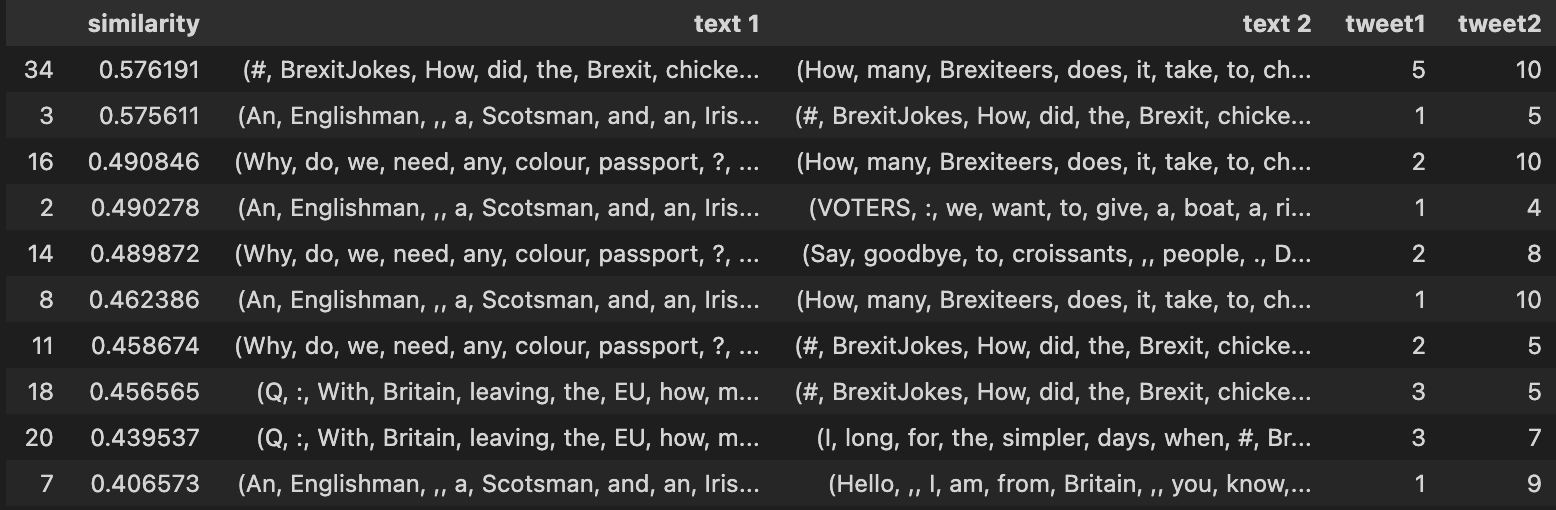
\includegraphics[width=15cm]{top_10_sim_doc.png}
		\caption{A table displaying the top ten similar tweets based on the whole tweet.}
		\label{fig:top_10_sim_doc}
		
	\end{figure}

	The information extraction process identified several interesting aspects from the tweets (see fig: \ref{fig:information_extract}). The results show that six of the tweet's sentiments scoring got classified as positive, and out of those six, five were in the top 5 results. We can't say for certain that having a positive tweet will likely score higher, as the dataset is not big enough to make that kind of claim. However, it does provide some good feedback and insights to the user. The NLP process also provided some excellent extraction of key phrases from the tweets. The only tweet's key phrase that didn't prove any meaningful information was Tweet 7's 'Brexit was'. Considering that these information extraction techniques, NER and key phrases, have not had any additional training, other than what comes out of the box, they have performed well in providing insights and feedback to the user.


	\begin{figure}[h]
		\centering
		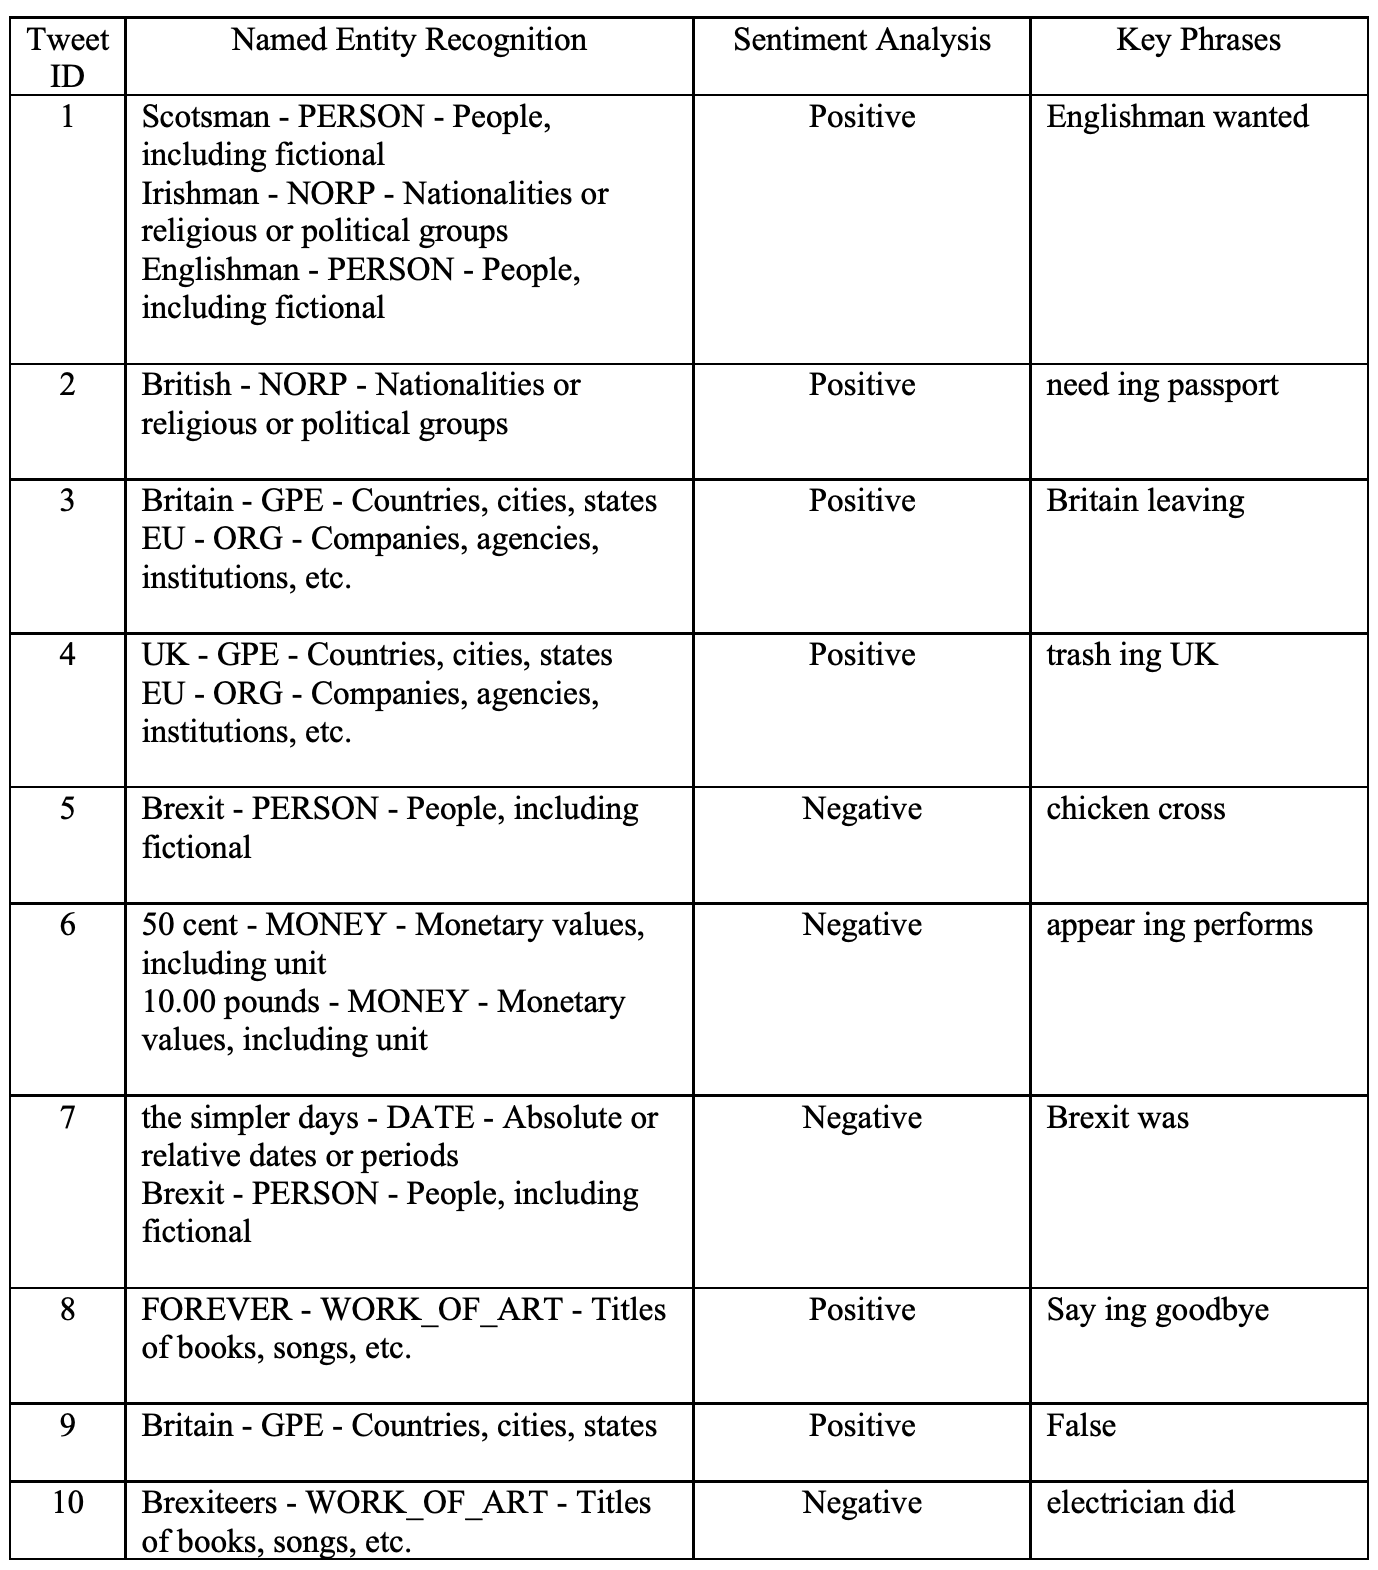
\includegraphics[width=10cm]{information_extract.png}
		\caption{A table displaying the key information extracted from the NER, Sentiment analysis and Key Phrases NLP processes.}
		\label{fig:information_extract}
		
	\end{figure}

	Using the TF-IDF, we extracted the key token features from all of the tweets. The higher the value, the more important that feature is for that tweet (see fig: \ref{fig:feature_extract}). However, this information does not provide much feedback for a user, but it would highly likely be adequate for training some form of ML models.

	\begin{figure}[h]
		\centering
		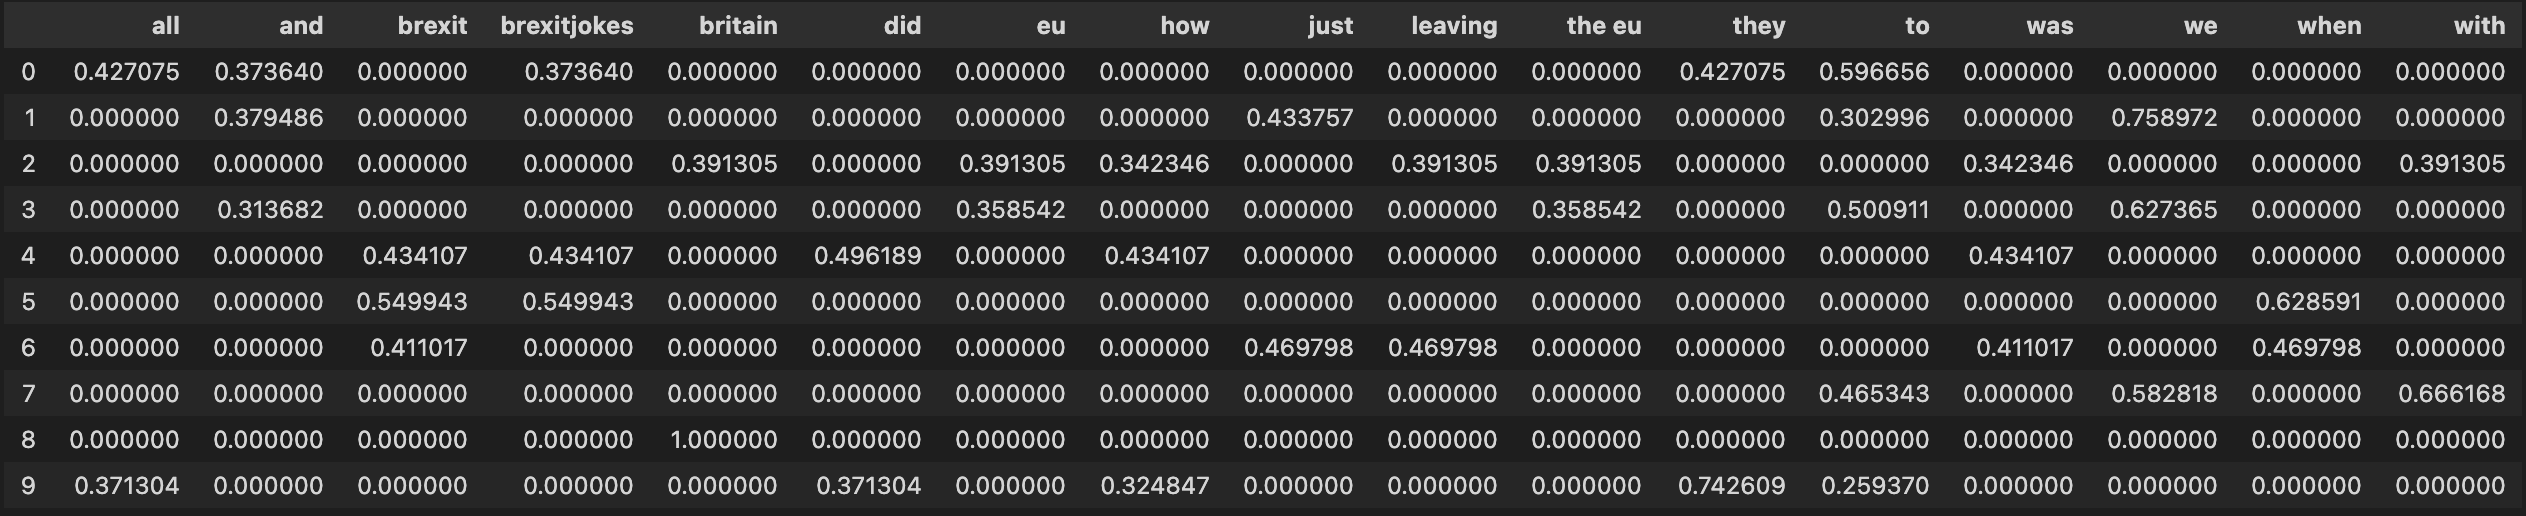
\includegraphics[width=\textwidth]{feat_extra_importance.png}
		\caption{A table showing the key tokens within each tweet and thir importance to that tweet.}
		\label{fig:feature_extract}
		
	\end{figure}

	In contrast, the information extraction techniques of finding word sequence patterns and utterance pattern matching did not provide any meaningful information. The finding word sequence pattern presented only "he'll appear" about Tweet 6, and the utterance pattern matching showed that a pattern was found in Tweet 6 too. These techniques have not provided much use currently but could be helpful when scaling up and using a much bigger dataset, like exam papers.



\section{Overall Results}
\label{sec:reaults_NLP}

	Overall we can suggest that the Elo ranking is a great alternative ranking system to the ACJ. It provides a robust scoring system because the combination process is random, removing any opportunity for Elo's flaws to be taken advantage of. It also provides the ability to try 'what if' calculations with potential comparison outcomes.
	
	On the other hand, the NLP information extraction provided some good information but was too basic to offer any real insights to the user to digest easily. While there is a lot of promise regarding the NLP, more fine-tuning is required to make this feature to provide feedback worthwhile. However, we believe this is a step worth taking with appropriate building blocks that have been put in place to expand upon.

